コンピュータは電子"計算機"であるから、計算を行うという目的に使うことも当然多い。だが、コンピュータでは、極限などのよう々な数学概念を扱うことができない(多項式の足し算などを行う"数式処理ソフトウェア"もあるが、これは数式を文字列として解釈し、その文字列に一定の処理を行なっているだけである)。そこで、式を扱うのではなく、数値そのものと四則演算を用いて計算を行うことになる。この計算方法が\textbf{数値計算法}\index{すうちけいさんほう@数値計算法}(numerical method)である。この章では、分野を問わずよく使われるであろう基礎的な数値計算法を紹介する。より多くの数値計算法を知りたい場合は、巷間に出まわる多数の参考書\footnote{一冊だけ挙げると、「Numerical Recipes in C」(W.H.Press et.al 著,丹慶他訳,1993,技術評論社)などが有名。}を参照されたい。

\section{1元方程式を解く}
まず、方程式$f(x)=0$の解を数値的に計算する初歩的な方法を学ぼう。以下、$f(x)=0$は区間$[a,b]$において唯一の実解を持つという前提で説明を記す。但し、実際には解を複数持ってもよい。つまり、図\ref{fig15_1}のような状況を思い描けば良い。
\begin{figure}[htb]
\centering
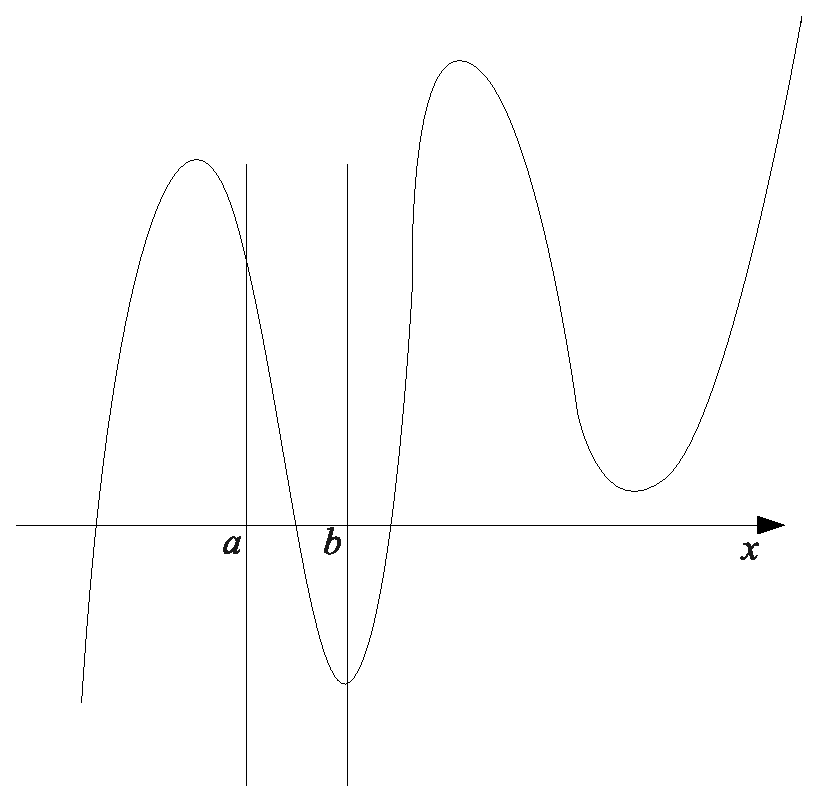
\includegraphics[width=0.5\linewidth,keepaspectratio]{fig15_1.eps}
\caption{方程式$f(x)=0$の様子}\label{fig15_1}
\end{figure}

複数の解を持つ場合は、区間を変えて解く事になる。つまり、このあと考えていくのは「区間内の1つの解を出す」方法である。

\subsection{逐次探索法}
方程式の解の存在がわかっているのであれば、「下手な鉄砲も数撃ちゃ当たる」という方針で、とにかく色々な値を代入してみれば良い。そのうち、方程式を満たす値が見つかるはずである。これを探索する方法の一つが\textbf{逐次探索法}\index{ちくじたんさくほう@逐次探索法}(serial search)である。

区間$[a,b]$の間を幅$h$で見ていく。つまり、$a,a+h,a+2h,\cdots,b$と代入して「解に近いもの」または解を探す。解が直接見つかればもちろんそれで良い。解そのものでなくとも、解の周辺では符号が変わることから、$f(a+kh)\cdot f(a+(k+1)h)<0$となるような場所が見つかるはずである。そこで、この区間$[a+kh,a+(k+1)h]$を、幅$h$をより小さくして再度探索する。これを繰り返していき、望みの精度になったら(小さい正数$\epsilon$に対して、$|f(x')|<\epsilon$となるような$x'$が見つかれば)それを解として出力すれば良い。

これは、解をリニアサーチしているのと同じ事である。計算時間がかかるので、通常はこのアルゴリズムが単独で用いられることはない。

\subsection{二分法}
先のように、解をリニアサーチしても良いのだが、区間が$[a,b]$に定まっていることを利用し、この間をバイナリサーチして解を見つけることもできる。この方法を\textbf{二分法}\index{にぶんほう@二分法}(bisection method)と呼ぶ。但し、$f(a)\cdot f(b)<0$が条件である。以下、手順を示しておく。
\begin{itembox}[l]{二分法}
\begin{enumerate}
\item $f\left(\frac{a+b}{2}\right)$を計算する。これが十分0に近ければ解として終了する。そうでなければ次項に進む。
\item $f(a),f(b)$のうち、先に計算した値と同符号の側の区間を縮める。例えば、$f(b)$が$f\left(\frac{a+b}{2}\right)$と同符号であれば、$b$を$\frac{a+b}{2}$で置き換える。置き換えた後、前項に戻る。
\end{enumerate}
\end{itembox}

\minisec{二分法+逐次探索法}
先に示した方法では$f(a)\cdot f(b)<0$が満たされない時などに使えない。そこで、前準備として逐次探索法を行い、適切な区間を定めてから二分法に切り替えることで高速に解を求めることもできる。
\begin{itembox}[l]{逐次探索付き二分法}
\begin{enumerate}
\item 区間$[a,b]$に対して逐次探索を行い、$f(x')\cdot f(y')<0$となるような$x',y'$を見つける。
\item $f\left(\frac{x'+y'}{2}\right)$を計算する。これが十分0に近ければ解として終了する。そうでなければ次項に進む。
\item $f(x'),f(y')$のうち、先に計算した値と同符号の側の区間を縮め(置き換え)て、前項に戻る。
\end{enumerate}
\end{itembox}

\minisec{二分法/逐次近似法の利用と注意}
ここまでの議論では解が区間$[a,b]$に唯一存在することを仮定しているが、実際にこれがわかっていることは稀だろう。従って、ここまでに紹介した方法はどちらかというと区間$[a,b]$を知る(解を囲い込む)ために用いられる。これらの方法を適用すれば、$f(x)$の符号の変わり目を知ることができ、中間値定理からその解の存在を伺える。

だが、逐次探索法・二分法共に解が充分近い場合はこれらを分離できないことがある。この場合、単純に区間幅を縮めても良いのだが、速度が遅くなり誤差も出やすくなるので、トレードオフとなる。他の方法の場合、これらの近い複数解のうち一つを見つけ出すことができるのに対し、逐次探索法や二分法ではうまくいかないのである。
\\ \\ 
逐次探索法・二分法には更に大きな欠点がある。それは、重解を検知できないことである。$(x-\pi)^2=0$という方程式が重解$\pi$を持つことは直ちにわかるが、この例のように無理数の重解を持つ場合、符号の変わり目がなく、「たまたま調べた場所が0になる」ことも少ないため、解が無いという事になってしまうのである。

その一方、これら2つの方法は急激な変化が起こる関数(例えば、"」"のような形をした関数)に対しても対応するという利点がある。
\\ \\ 
以上のように、方程式の解法は一つに絞るのではなく、様々な種類のものを状況に応じて使い分ける(時に併用する\footnote{実際、Brent法などでは何種類かの方法を状況に応じて戦略的に使い分けている。ソートでも、イントロソートは複数のソートを組み合わせていた。このように、アルゴリズムは状況に応じて適切に選択される必要があるものであり、一つ知っていればそれでいいという事はないのである。})べきなのである。

\subsection{割線法}
\textbf{割線法}\index{わりせんほう@割線法}(secant method)は図\ref{fig15_2}のように、仮の解$x_0,x_1$を定めておき、その2点を通る直線と$x$軸との交点を定め、それを次の「仮の解」$x_2$として、どんどん解を改良していく方法(総称して\textbf{反復法}\index{はんぷくほう@反復法}(iteration method)と呼ばれる)である。

\begin{figure}[htb]
\centering
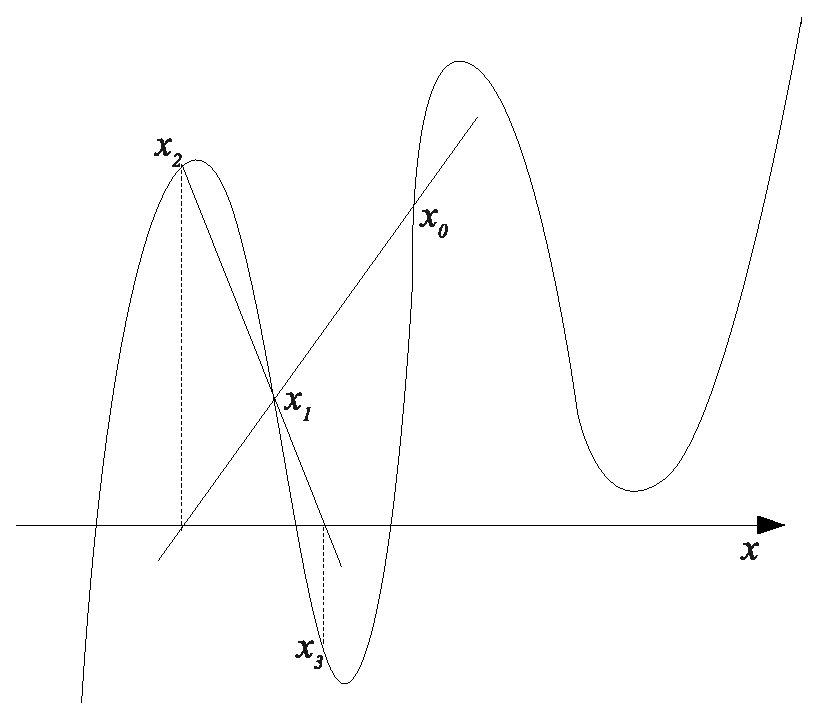
\includegraphics[width=0.5\linewidth,keepaspectratio]{fig15_2.eps}
\caption{割線法の様子}\label{fig15_2}
\end{figure}

\minisec{割線法の漸化式}
図\ref{fig15_2}は人間の目で見れば何をしているか直ちにわかる。だが、コンピュータは図から理解できるわけではないため、何らかの数式で表してやらなければならない。つまり、それまでの仮の解から、次の仮の解を数式によって決定しなければならないのである。以下、この漸化式を導出してみよう。
\\ \\ 
今、2つ前の仮の解が$x_{n-2}$であり、1つ前の仮の解が$x_{n-1}$であったとしよう。この時、この2点を通る直線の方程式は
\begin{equation}
y-f(x_{n-1})=\frac{f(x_{n-1})-f(x_{n-2})}{x_{n-1}-x_{n-2}}(x-x_{n-1})
\end{equation}
である。この直線と$x$軸との交点が$(x_n,0)$なのだから
\begin{equation}
-f(x_{n-1})=\frac{f(x_{n-1})-f(x_{n-2})}{x_{n-1}-x_{n-2}}(x_n-x_{n-1})
\end{equation}
である。これを$x_n$について解いて
\begin{equation}
x_n=x_{n-1}-\frac{x_{n-1}-x_{n-2}}{f(x_{n-1})-f(x_{n-2})}f(x_{n-1}) \label{secant}
\end{equation}
を得る。後は、この漸化式を順次計算すれば良いのである。以下、これを手順化しておく。
\begin{itembox}[l]{割線法}
\begin{enumerate}
\item 仮の解$x_0,x_1$を定める。また、$n=2$とする。
\item 式(\ref{secant})を用いて$x_n$を計算する。
\item 小さい正数$\epsilon$について、$|x_{n}-x_{n-1}|<\epsilon$か、$|f(x_{n})|<\epsilon$が満たされている場合はそれを解として終了する。そうでない場合、$n$を1増やして前項に戻る。
\end{enumerate}
\end{itembox}

\minisec{割線法の利用と注意}
割線法は必ずしも収束するとは限らない他、0に近い極値がある場合、それに影響されやすいという欠点を持つ。しかし、大抵の場合には(初期値さえ適切に選べば)きちんと解を出してくれるので、比較的使いやすい。一度やって収束しなくても、初期値を変えたら収束するような場合もありうるためである。だが、割線法は、複数解がある場合にどれを出すかわからないため、少し厄介である。

ここでは2点からの直線近似としたが、3点からの二次関数近似を利用して解を出す方法もある(Muller法)。Muller法は複素根も求められる優秀な方法であるが、その考えはここで紹介した割線法と原則同じである。そのため、割線法についてまず理解を深め、それから他の書籍などでMuller法を理解されると良いだろう。

\subsection{はさみうち法}
割線法は解を囲い込めないという欠点があった。そこで、囲い込み区間を決定し、その間の解を求められるように割線法を改良したのが\textbf{はさみうち法}\index{はさみうちほう@はさみうち法}あるいは\textbf{レギュラ・ファルシ法}\index{れぎゅらふぁるしほう@レギュラ・ファルシ法|see{はさみうち法}}(regula falsi method)である。
\begin{itembox}[l]{はさみうち法}
\begin{enumerate}
\item 仮の解$a,b$を定める。この時、$f(a)\cdot f(b)<0$を満たすものとする。これから探し求めるのは区間$[a,b]$の実解である。
\item 式(\ref{secant})において、$x_{n-1}=a,x_{n-2}=b$とおいて$x_{n+2}$を計算する。
\item $f(x_{n+2})$が十分0に近ければそれを解として終了する。そうでなければ、二分法同様に、$a,b$のうち符号の同じ側を$x_{n+2}$で置き換え、前項に戻る。
\end{enumerate}
\end{itembox}

はさみうち法は、割線法よりは収束が遅いが、解を囲い込めるのが利点である。初期値によっては二分法よりも遅いが、平均的にはこちらのほうがよく収束する。但し、重解に使えない点は同じである。

\subsection{Newton法}
割線法では2点をとり、それを直線近似することにより解を得た。だが、関数を直線で近似するときには、二点の平均変化率で近似するより各点の接線で近似したほうが正確になるだろう。この考えに基づくアルゴリズムが\textbf{Newton法}\index{Newtonほう@Newton法}ないし\textbf{Newton-Raphson法}と呼ばれるアルゴリズムである。重要なアルゴリズムであるので、まず使い方を述べた後、何種類かの導出を紹介し、その後実例となるソースを一つ見てみることにする。

\minisec{Newton法のアルゴリズム}
Newton法は、割線法と同様に仮の解を定めて、それを改良していく方法である。但し、割線法と違い、接線近似をするために仮の解は一つだけあれば良い。従って、Newton法で解を改良するための漸化式は二項間漸化式であり、次のように与えられる。
\begin{equation}
x_{n}=x_{n-1}-\frac{f(x_{n-1})}{f'(x_{n-1})} \label{Newton}
\end{equation}

この漸化式には何種類かの導出方法があり、後にその内の3種類を示す。先にその手順を示そう(ほとんど割線法と同じである)。

\begin{itembox}[l]{Newton法}
\begin{enumerate}
\item 仮の解$x_0$を定める。$n=1$としておく。
\item 漸化式(\ref{Newton})を用いて$x_n$を計算する。
\item 小さい正数$\epsilon$について、$|x_{n}-x_{n-1}|<\epsilon$か、$|f(x_{n})|<\epsilon$が満たされている場合はそれを解として終了する。そうでない場合、$n$を1増やして前項に戻る。
\end{enumerate}
\end{itembox}

漸化式(\ref{Newton})は収束しない場合がある。例えば、$x_{n+1}=x_{n-1}$となる場合や、極値周辺に落ち込んだ場合などに弱い。従って、ある程度収束の状況を見ておき、適切に収束しない場合は初期値を変えるなどの工夫をしなければならない。幸い、Newton法の収束はここまでに紹介した中でも一番速いので、やり直しても大した手間ではない。

また、関数の極値の大体の位置がわかっているならば、その$x_n$が極値の間から出た時にやり直す、などとすることで収束しやすくできる(上、区間を絞って解を見つけることもできる)。

\minisec{割線法の極限としての導出}
割線法は二点を通る直線によって計算を行う方法であった。この二点を近づけた時に得られる直線が接線になることは先刻承知であろう。従って、割線法の式(\ref{secant})の両辺について$x_{n-2}\rightarrow x_{n-1}$の極限をとった
\begin{equation}
x_n=\lim_{x_{n-2}\rightarrow x_{n-1}} \left(x_{n-1}-\frac{x_{n-1}-x_{n-2}}{f(x_{n-1})-f(x_{n-2})}f(x_{n-1})\right) \label{sec_newton}
\end{equation}
を計算してみる事で、Newton法を導出することができそうである。

ここで、
\begin{equation}
\lim_{x_{n-2}\rightarrow x_{n-1}} \frac{x_{n-1}-x_{n-2}}{f(x_{n-1})-f(x_{n-2})}=\lim_{x_{n-2}\rightarrow x_{n-1}} \frac{1}{\frac{f(x_{n-2})-f(x_{n-1})}{x_{n-2}-x_{n-1}}}=\frac{1}{f'(x_{n-1})}
\end{equation}
である。このことから、式(\ref{sec_newton})は
\begin{equation}
x_n=x_{n-1}-\frac{f(x_{n-1})}{f'(x_{n-1})}
\end{equation}
となり、たしかに式(\ref{Newton})と一致する。
\\ \\ 
以上のように、Newton法は割線法の極限として見ることができる。逆に、微分を差分近似することで割線法に戻すことも可能である(これについては後に述べる)。

\minisec{接線近似からの導出}
先の方法では、平均変化率を求めてから極限を取ることにした。だが、最初から接線を計算すればそれで問題なく導出することができる。釈迦に説法かもしれないが、ここで接線を用いて導出しておこう。

点$(x_{n-1},f(x_{n-1}))$を通る接線の方程式は
\begin{equation}
y-f(x_{n-1})=f'(x_{n-1})(x-x_{n-1})
\end{equation}
である。この接線と$x$軸の交点の$x$座標が$x_n$であるので
\begin{equation}
-f(x_{n-1})=f'(x_{n-1})(x_n-x_{n-1})
\end{equation}
となる。これを解くことで、式(\ref{Newton})が導かれる。
\\ \\ 
先の割線法からの導出は割線法との関係がよく見える方法である。だが、このように接線近似を行ったほうが手早く導出できる。漸化式(\ref{Newton})を忘れた時にはこの方法で導出するのが一番手っ取り早いだろう。

\minisec{解析的導出}
Newton法はTaylor展開を用いた微分近似によっても求められる。この方法は別の解法の導出の際にも用いられるため、ここでNewton法を例にして紹介しておくことにする。

$f(x)$を$x=x_n$でTaylor展開すると
\begin{equation}
f(x)=f(x_n)+f'(x_n)(x-x_n)+\cdots
\end{equation}
となる。この右辺の二次以上の項を落として$f(x)$を一次近似すると
\begin{equation}
f(x)\approx f(x_n)+f'(x_n)(x-x_n)
\end{equation}
となる。ここから、右辺=0の解を求めれば
\begin{equation}
x=x_n-\frac{f(x_{n})}{f'(x_{n})}
\end{equation}
となる。後は、これを順次適用していけば解に近づいていくだろうことから、$x$を$x_{n+1}$で置き換えれば、たしかに式(\ref{Newton})を得られる。

このように、方程式を(必要に応じて近似を行い)変形して左辺と右辺にわけ、右辺を既知項・左辺を未知項として漸化式を導出するのは、反復法において非常によく使われる導出法である。
\\ \\ 
途中、Taylor展開で二次以上を落としたが、二次項まで残すとまた別の解法になる。

\minisec{数値微分との併用}
Newton法の漸化式には、求めたい方程式の導関数がある。導関数が簡単に求まればいいのだが、そうは行かない場合もあるだろう。そこで、コンピュータを用いて数値的に微分を計算(\textbf{数値微分}\index{すうちびぶん@数値微分}(numerical differentiation))してしまえば良いのでは?という考えに至る。

コンピュータで微分を計算する場合、基本となるのは差分近似である。以下、Taylor展開を用いて、1階微分の\textbf{前進差分近似}\index{ぜんしんさぶんきんじ@前進差分近似}(forward difference)と、\textbf{中央差分近似}\index{ちゅうおうさぶんきんじ@中央差分近似}(centered difference)を導出してみよう。

Taylor展開より、十分小さい$h$について、
\begin{equation}
f(x+h)=f(x)+hf'(x)+\cdots \label{taylor}
\end{equation}
である。ここまではどちらの微分近似の導出も同じである。
\\ \\ 
前進差分近似では、式(\ref{taylor})の二次以上の項を落として、$f'(x)$について解く。すると、
\begin{equation}
f'(x)\approx \frac{f(x+h)-f(x)}{h} \label{forward}
\end{equation}
となる。この時の打ち切り誤差は、二次以上の項を落として$h$で割っているので、$O(h)$である。
\\ \\ 
中央差分近似では式(\ref{taylor})を用いて、$f(x+h)-f(x-h)$を計算する。これにより、右辺は奇数次の項しか残らない。
\begin{equation}
f(x+h)-f(x-h)=2hf'(x)+\cdots
\end{equation}
ここで、三次以上の項を落として$f'(x)$についてとけば
\begin{equation}
f'(x)=\frac{f(x+h)-f(x-h)}{2h} \label{centered}
\end{equation}
を得る。この誤差は$O(h^2)$である。
\\ \\ 
今、式(\ref{forward})を用いてNewton法の計算を行うことを考えよう。式(\ref{Newton})に式(\ref{forward})を代入して
\begin{equation}
x_{n}=x_{n-1}-\frac{hf(x_{n-1})}{f(x_{n-1}+h)-f(x_{n-1})}
\end{equation}
を得る。これは、微分を差分化しているので割線法と同様の形式である。つまり、Newton法に前進差分を適用すると割線法に帰着するという事である。これは何も前進差分に限った話ではない。中央差分近似を始めとする他の方法を使ったとしても、割線法と本質的には同じアルゴリズムになる(平均変化率の計算が少し変わるだけ)。

ここで述べた方法によりNewton法に数値微分を組み合わせた場合、割線法を(任意の幅で)用いる場合に比べて収束が遅い場合が多い為、これを使うぐらいなら最初から割線法で攻めたほうが良いだろう。しかし、割線法とNewton法の関係が、差分と微分の関係であることを理解するのに重要なことであるため、ここで述べた。
\\ \\ 
なお、蛇足ながら、数値微分の差分近似方法はここに紹介した以外にも沢山あり、Taylor展開から導出できる。例えば、$f(x+h)+f(x-h)$から二階微分の公式が導出できる他、$f(x),f(x\pm h),f(x\pm 2h)$を用いて一階微分を計算することにより、より精度の良い公式が導出できる。興味があれば計算してみていただきたい。

\minisec{Newton法の実例〜平方根の計算〜}
ここまでで、Newton法の素性について学習したので、これを実際に使って正平方根を計算する関数を作成してみることにしよう。
\\ \\ 
ソースコードの前に、Newton法の漸化式をどう書けばいいか考えておく。数$a$の正平方根$\sqrt{a}$を解に持つ方程式のうち、$x$と$a$及び定数だけで簡単に書けるものとして
\begin{equation}
x^2-a=0
\end{equation}
という方程式が挙げられる。これをNewton法により解く。

$f(x)=x^2-a$として、式(\ref{Newton})を書き下すと
\begin{equation}
x_{n}=x_{n-1}-\frac{x_{n-1}^2-a}{2x_{n-1}}
\end{equation}
である。初期値は、正の値ならば(その形状を推測して)何でも良いが、ここでは決めやすく$a$としておこう。これにより、Newton法を書く準備ができたので、以下に引数の正平方根を計算する関数を実装してみることにする。
\begin{boxnote}
\begin{multicols}{2}
\minisec{Newton法による平方根の計算}
Newton法を用いて引数の正の平方根を計算する関数\verb|newton_sqrt|を実装してみる。ここでは、収束の判定を、解候補の二乗と元の数の差が$10^{-6}$未満であるとし、マクロ\verb|EPS|によって定めるものとした。なお、収束しない場合の処理などは行なっていない。
\begin{lstlisting}[caption=Newton法による開平,label=program15_1]
#include<math.h>
#define EPS 1E-6

double newton_sqrt(double a){
  double x=a;
  do{
    x-=(x*x-a)/(2*x);
  }while(fabs(x*x-a)>=EPS);
  return x;
}
\end{lstlisting}
\end{multicols}
\end{boxnote}

このように、解を求めることができる方程式に対しても、その解の数値の計算のためなどの理由で、数値解法を用いる場合があるのである。

\section{数値積分法}
ある定積分を数値的に計算する。積分は面積であるから、その面積を何らかの近似で求められれば良い。この時、区間を大きく取ると近似しづらくなるので、
\begin{equation}
\int^{b}_{a} f(x)=\sum^{n-1}_{k=0}\int^{x_{k+1}}_{x_k}f(x)dx \ \quad(x_0=a,x_n=b) \label{integrals}
\end{equation}
のように区間に分割して計算を行う。数列$\{x_n\}$を$x_{n+1}=x_n+h$として決めれば、これは等分割になることがわかるだろう。ここでは、このような等分割の場合\footnote{ガウス・ルジャンドルの積分公式など等分割にしない方法も存在する。}に、右辺の積分をどのように近似するかを見ていくことにする。最後に、少し違ったアプローチでの積分方法を紹介する。

\subsection{台形則}
以前の講義で既に紹介したが、\textbf{台形則}\index{だいけいそく@台形則|see{台形積分}}ないし\textbf{台形積分}\index{だいけいせきぶん@台形積分}公式は、式(\ref{integrals})右辺の積分を台形によって近似し
\begin{equation}
\int^{x_{k+1}}_{x_k}f(x)dx=\int^{x_k+h}_{x_k}f(x)dx\approx \frac{h}{2}\left(f(x_k)+f(x_k+h)\right)
\end{equation}
と近似する方法である。

\subsection{中点則}
\textbf{中点則}\index{ちゅうてんそく@中点則}(midpoint integral)は、区間分割の近似を台形ではなく長方形で行う方法である。この時、長方形の幅が$h$であることはすぐにわかるが、高さには幾つかの選び方がある。$f(x_k)$や$f(x_k+h)$を高さにする方法は高校などで区分求積法として説明されるが、中点則ではその名前通り、中点を高さにとる。つまり、$f(x+0.5h)$を高さの基準として用いる。これにより、式(\ref{integrals})右辺の積分は
\begin{equation}
\int^{x_{k+1}}_{x_k}f(x)dx=\int^{x_k+h}_{x_k}f(x)dx\approx hf(x_k+0.5h)
\end{equation}
と簡単に近似できる。
\\ \\ 
通常、数値積分では台形則の方がよく用いられるが、このような方法があることも知っておくと良い。

\subsection{シンプソン則}
\textbf{シンプソン則}\index{しんぷそんそく@シンプソン則}(Simpson integral)は古典的な積分公式として知られている方法である。台形則よりも時間がかかるため精度が必要ない場合には使われず、精度が必要な場合はローンバーグ積分やガウス・ルジャンドル積分の方が有用であるのでやはり使われないという、博物館行きになった感のある公式である。とはいえ、初歩として知っておく価値はあるので、ここでその概要を紹介しておこう。

$x_k,x_k+0.5h,x_k+h$から、関数を二次関数で近似することを考える。ただし、この形式で書くのは面倒であるので、$x'_-=x_k,x'=x_k+0.5h,x'_+=x_k+h$および$h'=0.5h$とおいて議論を進める(こちらのほうが一般的な形になるため)。また、$f'_-=f(x'_-),f'_+=f(x'_+),f'=f(x')$とする。
\\ \\ 
三点を通る二次関数$g(x)$は唯一に定まる。そこで、(簡単のため)二次関数を
\begin{equation}
g(x)=a(x-x')^2+b(x-x')+c
\end{equation}
とおき、これが3点を通るように$a,b,c$を定めることとする。単純に各点を代入して解けば
\begin{equation}
\left(a,b,c\right)=\left(\frac{f'_-+f'_+-2f'}{2h'^2},\frac{f'_+-f'_-}{2h'},f'\right) \label{simpson1}
\end{equation}
となる。一方、
\begin{equation}
\int g(x)dx=\frac{a}{3}(x-x')^3+\frac{b}{2}(x-x')^2+cx \label{simpson2}
\end{equation}
である(ただし、積分定数を省いた)。

式(\ref{simpson2})に式(\ref{simpson1})を代入して整理し、定積分の形に書き直すと
\begin{equation}
\int^{x'_+}_{x'_-}f(x)dx\approx \int^{x'_+}_{x'_-}g(x)dx=\frac{h'}{3}[f'_-+4f'+f'_+]
\end{equation}
を得る。これが、シンプソン則である。
\\ \\ 
シンプソン則を用いる場合は、先のように中点を用いる場合もあるし、3点ずつ適用するように変える方法もある。

\subsection{モンテカルロ積分}
\textbf{モンテカルロ積分}\index{もんてかるろせきぶん@モンテカルロ積分}(Monte Carlo integral)は、ここまでの方法とは変わった形で積分を行う方法で、とりわけ多次元積分や解析的に書きにくい領域の面積を求めるのに用いられる。なお、一般のアルゴリズムで\textbf{モンテカルロ法}\index{もんてかるろほう@モンテカルロ法}(Monte Carlo method)と言った場合、乱数を用いて計算を行うアルゴリズムで、それ故に結果が正しいとは限らないもののことを言う\footnote{これに対し、乱択クイックソートのように、乱数を使うがゆえに時間が一定に定まらない(解は正しく出る)ものを\textbf{ラスベガス法}\index{らすべがすほう@ラスベガス法}(Las Vegas method)と呼ぶ。}。ここで挙げたモンテカルロ積分もモンテカルロ法の一種である。
\\ \\ 
積分したい領域を図\ref{monte}のように長方形で囲む。そして、囲んだ領域に対し、一様乱数を用いて\footnote{これがどの程度一様か、と言う所で正確性が定まる。計算向けにはC言語の標準関数のrandを用いるよりも、メルセンヌ・ツイスターと呼ばれる方法を用いたほうが良い。}点を「撒く」。そして、このうち幾つの点が領域内に入っているか、その割合を出せば囲んだ領域の近似となるだろう。
\begin{figure}[htb]
\centering
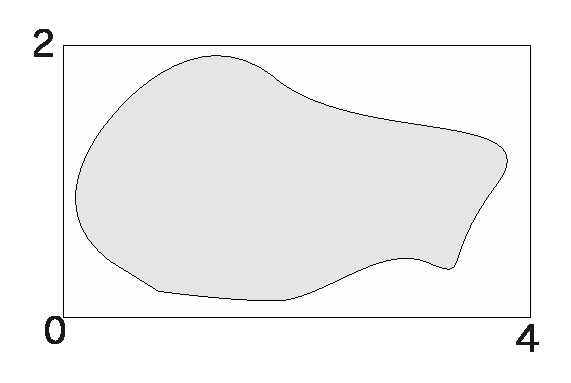
\includegraphics[width=0.6\linewidth,keepaspectratio]{fig15_3.eps}
\caption{モンテカルロ積分したい領域の様子(灰色領域)}\label{monte}
\end{figure}

この近似方法を手順にしてまとめておこう。
\begin{itembox}[l]{二次元のモンテカルロ積分}
\begin{enumerate}
\item 計算したい領域を長方形で囲む。また、$c=0$とする。
\item 次の2つの操作を$n$(任意の自然数値)回繰り返す。
\begin{enumerate}[(1)]
\item 長方形内の点を一点、一様乱数を用いて選ぶ。
\item 選んだ点が積分領域内に入っているかどうかを判定し、入っている場合は$c$を1増やす。
\end{enumerate}
\item 長方形の面積$\times c/n$を計算し、それを積分値とする。
\end{enumerate}
\end{itembox}

この方法は、3次元の場合でも長方形を直方体に変えるだけで実行できるので、多次元積分に使いやすい。また、積分領域が解析的に書き表しにくい場合でも、領域として判定できさえすればいいので、台形積分が使えない場合などでも使えるという利点がある。
\\ \\ 
モンテカルロ積分の精度は、$n$が十分大きいならば、寧ろ一様性による。つまり$n=2^{16}$であるのを$n=2^{20}$に増やすよりも、乱数がより一ように出るようにしたほうが精度が良くなる。十分良い規則があるならば、点を選ぶのに乱数を用いず、規則性を用いて一様性を確保することもできる(\textbf{準モンテカルロ積分}\index{じゅんもんてかるろせきぶん@準モンテカルロ積分}(semi-Monte Carlo integral)と呼ぶ)。だが、例えば細かい波状の境界の場合などは、適切な規則性が見当たらず、乱数を用いて選んだほうが適切に点を選べる場合もある。

\section{連立方程式と行列}
多元一次連立方程式を解く際に行列を用いる方法については既知であろう。この行基本変形をシステマティックに行うことによって、数値的に連立方程式の解を得ることができる。連立方程式を解くことは、数値計算の各所で必要になる操作であるため、ここでその基本を紹介しておく。また、その簡単な応用として、逆行列や行列式を求める方法についても触れる。なお、ここで紹介する方法についてのライブラリを作成するのは、配列・構造体・ポインタなどの良い復習になるので、できれば汎用ライブラリとしてまとめてみると良い。
\subsection{Gauss法}
\textbf{Gauss法}\index{Gaussほう@Gauss法}(Gaussian Elimination)は、連立方程式を解く方法では最もポピュラーな方法であり、前進消去過程と後退代入過程からなる。

\minisec{前進消去過程}
連立方程式を表すため、以下、$n$行$n+1$列からなる拡大係数行列$A$を考える。もちろん、第$n+1$列は連立方程式の定数ベクトルである。また、$a_{i,j}$と書いた場合、これは行列$A$の$i,j$成分を指すものとする。
\\ \\ 
拡大係数行列の下三角成分を0にする過程が前進消去過程である。前進消去過程では、第$k$行を用いて第$k+1$行以降の各行の第$k$列成分を0にする。これを$k=1$から順にやることで、下三角成分を0にすることができる。手順をまとめておこう。
\begin{itembox}[l]{Gauss法の前進消去過程}
\begin{enumerate}
\item $k=1$としておく。
\item $i=k+1,k+2,\cdots$及び$j=k+1,k+2,\cdots$として、次の計算を行う(ただし、$-=$はC言語の\verb|-=|と同じ意味)。
\begin{equation}
a_{i,j}-=\frac{a_{i,k}}{a_{k,k}}a_{k,j} \label{gauss1}
\end{equation}
\item $k=n$であれば終了する。そうでなければ、$k$を1増やし、前項に戻る。
\end{enumerate}
\end{itembox}

なお、実際の計算では、下三角が0になることはわかっているので、影響がある上三角部分だけ計算するようにしている。

以上により前進消去過程が行われたら、続いて後退代入過程を施し、連立方程式を解く。

\minisec{後退代入過程}
前進消去が行われた状態では、一番下(第$n$行)は単なる一次方程式になっている。そこで、これを解くことで、解のうちの一つを求めることができる。求めた解を、一つ上(第$n-1$行)に代入して計算すれば、解成分がもうひとつ明らかになる。このように、下側から代入して解を求める…を繰り返すことで、連立方程式の解を求めることができる。これが、後退代入過程である。
\begin{itembox}[l]{Gauss法の後退代入過程}
\begin{enumerate}
\item $k=n$としておく。また、$x_i$は解ベクトルの第$i$成分とする。
\item 次の式により、$x_k$を求める(ただし、$k=n$の時には総和部分は計算されない)。
\begin{equation}
x_k=\frac{1}{a_{k,k}}\left(a_{k,n+1}-\sum^{n}_{i=k+1}a_{k,i}x_{i}\right) \label{gauss2}
\end{equation}
\item $k=1$であれば終了する。そうでなければ、$k$を1減らし、前項に戻る。
\end{enumerate}
\end{itembox}

なお、この方法を用いるときに、総和を逐次求めるのではなく、$x_k$がわかった時にそこから上の行について減算を行なっておくという実装もできる。
\\ \\ 
実際には、ここまでに述べた前進消去と後退代入をあわせてGauss法と呼んでおり、これらは一連の作業である。だが、分けたほうがこのあとの説明に便利であるため、2つに分けて説明した。

\minisec{部分ピボット選択}
前進消去過程の式(\ref{gauss1})においては、割り算を伴うため、0による除算をしないように気をつけなければならない。だが、計算過程において$a_{k,k}$が0になってしまう場合は十分にありうる。こんな時に行うのが\textbf{ピボット選択}\index{ぴぼっとせんたく@(連立方程式の)ピボット選択}(pivot selection)である。ここで、ピボットというのは$a_{k,k}$のように、行/列とも同じ番号の成分のことを言う。

もしもピボット$a_{k,k}$が0になってしまった場合(あるいは絶対値が非常に小さい場合)、そこから下の行を見ていき、0でない成分$a_{j,k}$($j>k$)を探し求める。適切な$j$が見つかったら、第$k$行と第$j$行を入れ替える\footnote{蛇足ながら、浅いコピーを用いたほうが速度が速くて良い。}。このような行交換を行う方法が\textbf{部分ピボット選択}である。なお、行交換に加えて列交換も行う\textbf{完全ピボット選択}もあるのだが、ここでは名前だけの紹介に留める。
\\ \\ 
部分ピボット選択は、0による除算の回避のためだけにあるのではない。実際は、小さい値による割り算を行うと誤差が出たりする場合があるため、それを緩和する役目も持っている。一般には、同じ列の成分のうち、最も絶対値の大きい値をピボットに持ってくると良いとされる。これを含めて、前進消去過程を書き換えよう。
\begin{itembox}[l]{部分ピボット選択付き前進消去}
\begin{enumerate}
\item $k=1$としておく。
\item $a_{i,k}\ (i\ge k)$のうち、絶対値が最も大きい値を求める($a_{m,k}$とする)。求めた$m$に対し、$m$行と$k$行を交換する。
\item $i=k+1,k+2,\cdots$及び$j=k+1,k+2,\cdots$として、式(\ref{gauss1})の計算を行う。
\item $k=n$であれば終了する。そうでなければ、$k$を1増やし、前々項に戻る。
\end{enumerate}
\end{itembox}

なお、部分ピボット選択の過程において、ある列で0の要素しか見当たらなくなった場合、その連立方程式には解が存在しないか、解が無数にある。この判定ができることも含めて、連立方程式を解く際には部分ピボット選択をつけておくと良い。

\minisec{LU分解}
同じ係数行列でありながら、定ベクトルが異なる複数の連立方程式を解くことがある。このような場合に高速化を図る手法が\textbf{LU分解}\index{LUぶんかい@LU分解}(LU decomposition)である。ここでは、数学的な議論は割愛し、プログラミングの観点からLU分解を扱う。
\\ \\ 
同じ係数行列・異なる定ベクトルであれば、前進消去過程の大半(定ベクトルに対する計算以外の部分)は無駄である。従って、何とかしてこの無駄な部分を省くことはできないか、と考えてみる。

定ベクトルの計算に必要なのは、消去の時に、その行を何倍して引いたかという情報だけである。つまり、各過程における$\frac{a_{i,k}}{a_{k,k}}$さえわかれば、後は定ベクトルを計算することができる。従って、$\frac{a_{i,k}}{a_{k,k}}$を記録しておこう、という事になる。この時、行列の下三角成分は無益に残っているだけなので、そこにメモすれば良い。これを手順化すると、次のようになる。
\begin{itembox}[l]{行列のLU分解}
以下、拡大係数行列ではなく、$n\times n$の係数行列を考えるものとする(ピボット選択は省いたが、省かずとも同じ手順である)。
\begin{enumerate}
\item $k=1$としておく。
\item $i=k+1,k+2,\cdots$及び$j=k+1,k+2,\cdots$として、式(\ref{gauss1})の計算を行う。更に、この時の$\frac{a_{i,k}}{a_{k,k}}$の値を$a_{i,k}$に保存しておく。
\item $k=n$であれば終了する。そうでなければ、$k$を1増やし、前項に戻る。
\end{enumerate}
\end{itembox}

一度上記の手順を踏んで計算すれば、後は次の手順で(異なる定ベクトルに対しても)解を求められる。
\begin{itembox}[l]{LU分解後の解の計算}
以下、定ベクトルの第$i$成分を$b_i$と記す。
\begin{enumerate}
\item $k=1$としておく。
\item $i=k+1,k+2,\cdots$とし、$b_i$から$a_{i,k}\cdot b_k$を引く。
\item $k=n$ならば次項へ進む。そうでなければ$k$を1増やして前項に戻る。
\item 後退代入過程を行い、解を計算する。
\end{enumerate}
\end{itembox}

「その方程式を解くのは一度限り!」という場合を除いては、この方法により計算すれば同じ計算を省略することが出来る。

\subsection{Gauss-Jordan法}
\textbf{Gauss-Jordan法}\index{Gauss-Jordanほう@Gauss-Jordan法}はGauss法よりも少し遅いが、間違えづらい方法で、特に逆行列への応用が効きやすい方法である。なお、ここでもやはり拡大係数行列を用いて説明を行う。
\\ \\ 
Gauss-Jordan法は、係数行列に行基本変形を行い、単位行列に変換することによって連立方程式を解く方法である。早速手順を見てみよう(部分ピボット選択を含んでいる)。
\begin{itembox}[l]{Gauss-Jordan法}
\begin{enumerate}
\item $k=1$としておく。
\item $a_{k,k}$が0である場合、$a_{i,k}\neq0\ (i>k)$を満たす行を見つけ、第$i$行と第$k$行を交換する。
\item 第$k$行の全ての成分を$a_{k,k}$で割っておく。これにより、$a_{k,k}=1$となる。
\item $i\neq k$なる全ての$i$に対し、第$i$行から($a_{i,k}\times$第$k$行)を引く。
\item $k=n$ならば終了する。そうでなければ$k$を1増やし、ステップ2に戻る。
\end{enumerate}
\end{itembox}

この変形により、係数行列は単位行列になり、定ベクトル(拡大係数行列の第$n+1$列)は解ベクトルそのものになっている。
\\ \\ 
この方法はGauss法に比べて実装が楽なので、しばしば、連立方程式の解を出すアルゴリズムの試験のために用いられる。

\subsection{行列式や逆行列への応用}
Gauss法やGauss-Jordan法は行基本変形を元にしているため、他の行列操作にも応用できる。ここでは、Gauss法を行列式に、Gauss-Jordan法を逆行列に応用してみよう。

\minisec{Gauss法による行列式の計算}
行列式の計算を行う場合、第1列の成分のうち第1行以外を0にすれば、これが定数となって出てくる。すなわち、
\begin{equation}
\left|
\begin{array}{ccc}
a_{1,1}&\cdots&a_{1,n}\\
0&\cdots&a_{2,n}\\
\vdots&\ddots&\vdots\\
0&\cdots&a_{n,n}
\end{array}
\right|=a_{1,1}\left|
\begin{array}{ccc}
a_{2,2}&\cdots&a_{2,n}\\
\vdots&\ddots&\vdots\\
a_{n,2}&\cdots&a_{n,n}
\end{array}
\right|
\end{equation}
とできる。ここで、$a_{k,k}$を用いてそこから下の成分を0にするのは、Gauss法の前進消去過程そのものであることを思い出せば、前進消去の際にピボットを随時掛け算していくことによって行列式の値を計算することができることがわかるだろう。

\minisec{Gauss-Jordan法による逆行列の計算}
係数行列と単位行列をくっつけた
\begin{equation}
\left[
\begin{array}{ccc|ccc}
a_{1,1}&\cdots&a_{1,n}&1&\cdots&0\\
\vdots&\ddots&\vdots&\vdots&\ddots&\vdots\\
a_{n,1}&\cdots&a_{n,n}&0&\cdots&1
\end{array}\right]
\end{equation}
を用意し、これに対してGauss-Jordan法を適用すると逆行列を得ることができる。これは、Gauss法でも同じ事である。特段説明することはないだろう。
\\ \\ 
注意すべき点として、この方法で逆行列を求めてから連立方程式を解くと、速度が遅く、誤差も大きくなりがちである。これは、連立方程式に限ったことではない。例えば、$x_{k+1}=A^{-1}x_k$のような漸化式がある場合、$Ax_{k+1}=x_k$と変形してLU分解を用いたほうが逆行列を計算するよりも(特に誤差の面で)良い結果が得られる。従って、この方法で逆行列を得るのは、あくまでも逆行列そのものに興味がある場合と考えて良い。
\\ \\ 
実は、この方法は逆行列を得る方法としても最適のものではない。実際には、「第$i$成分が1で他は0」という解ベクトルを$i=1,\cdots,n$として用意し、LU分解を用いて解いたほうが良い。実際に計算回数を見積もってみていただきたい。

\newpage

\begin{shadebox}
\section*{本講の要点}
本講では、分野を問わずよく使われるであろう基礎的な数値計算法を学んだ。

\subsection*{一元方程式の解法}
\begin{itemize}
\item 代数方程式の解を数値的に出す場合、一度に全ての解を出すことは通常難しいため、区間を絞って一つずつ出していくことになる。
\item 区間をリニアサーチするのが逐次探索法、二分探索するのが二分法である。
\item 割線法は曲線上の2点をとり、それらを結ぶ直線を引いて$x$軸との交点を求めるという操作を繰り返すことで解を求める方法である。
\item 割線法に、二分法と似たような区間制限をつけたのがはさみうち法である。
\item 割線法の極限として、接線を用いて近似したのがNewton法である。
\end{itemize}

\subsection*{数値積分法}
\begin{itemize}
\item 数値積分を行う場合は通常、小区間に分割し、その各区間を近似的に計算して総和を求める形で積分する。
\item 台形則は台形・中点則は中点の高さの長方形で区間を近似する。
\item シンプソン則は関数上に3点をとり、そこを二次関数近似することによって積分を計算する。
\item モンテカルロ積分は、領域の面積を求めるのに適した方法で、点を「撒いて」、それが求めたい領域に入った割合によって計算する方法である。
\end{itemize}

\subsection*{連立方程式と行列}
\begin{itemize}
\item Gauss法は下三角成分を0にする前進消去過程と、それによって解を順次求めていく後退代入過程からなる。
\item Gauss-Jordan法は係数行列を単位行列に変換することによって解を求める方法である。
\item 同じ係数行列に対して前進消去過程を繰り返すのは無意味であるので、それをメモしておいて複数の定ベクトルに使いまわす方法がLU分解である。
\item 行基本変形のうち、行交換の過程のことを部分ピボット選択と呼んでいる。
\item 連立方程式を解くアルゴリズムは、逆行列や行列式の値を求める際に容易に応用できる。
\end{itemize}

\end{shadebox}
